%"###############################################
%
% Classification supervisée
%
%###############################################

% RTUPB: variables post-op à 12 mois
%
%###############################################

Dans les sections qui suivent, nous réutilisons la même méthode pour construire un arbre de régression:
pour chacune des techniques opératoires (respectivement RTUPB, VPPBS et VAPOR) et à partir des données pré-opératoires précédemment utilisées et nettoyées des variables invariantes ou incomplètes, auxquelles on ajoutera
la variable à prédire, nous effectuons un tirage aléatoire pour créer deux ensembles de données:
\begin{itemize}
\item un ensemble d'apprentissage représentant 80\% des patients opérés par une technique. A partir de cet ensemble, nous inférerons un arbre de régression en utilisant le package rpart sous R.
\item un ensemble de validation représentant 20\% des patients opérés par la même technique.
\end{itemize}
Les variables IPSS et QoL seront traitées comme des variables ordinales, tandis que la variable Qmax sera
traitée comme une variable linéaire.

\subsubsection{RTUPB: QoL à 12 mois}

L'arbre de régression obtenu pour la variable QoL à 12 mois (colonne QoL\_\_4) met en \{oe}uvre une seule variable (Cf. figure~\ref{fig-rtupb-regtree-qol12}). Les feuilles de l'arbre représentent, en première ligne, la valeur prédite (la plus probable) pour QoL à 12 mois. La ligne suivante indique les probabilités pour chacun des 3 niveaux constatés sur l'échantillon d'apprentissage pour QoL à 12 mois, c'est-à-dire respectivement 0/1/2. Par exemple en cas d'IPSS pré-opératoire à 30, l'arbre de régression conduit à la feuille en bas à droite et prédit une valeur QoL à 2 avec une probabilité de 53\%.

Nous vérifions le rôle et le poids d'autres variables dans cet arbre de régression:
\begin{lstlisting}[language=R]
> dt$variable.importance
              IPSS P.O              Age (ans) Délai ablation (jours) 
              3.710944               2.061636               2.061636 
               QoL P.O             Anesthésie        Qmax P.O (ml/s) 
              2.061636               1.649308               1.649308 
\end{lstlisting}


\begin{figure}[H]
\centering
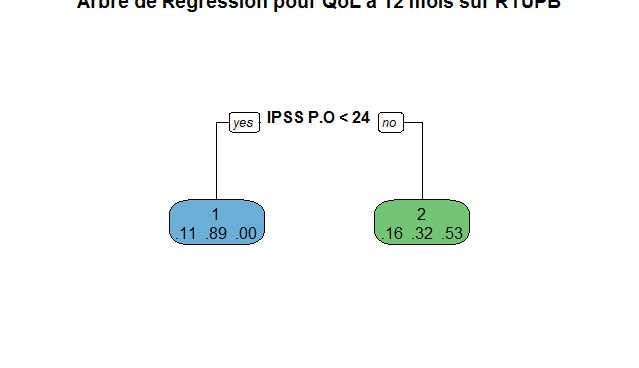
\includegraphics[width=0.75\textwidth]{../Fig/RTUPB/rtupb-regtree-qol12.png}
\caption{RTUPB: Arbre de régression pour QoL à 12 mois}
\label{fig-rtupb-regtree-qol12}
\end{figure}

\begin{figure}[H]
\centering
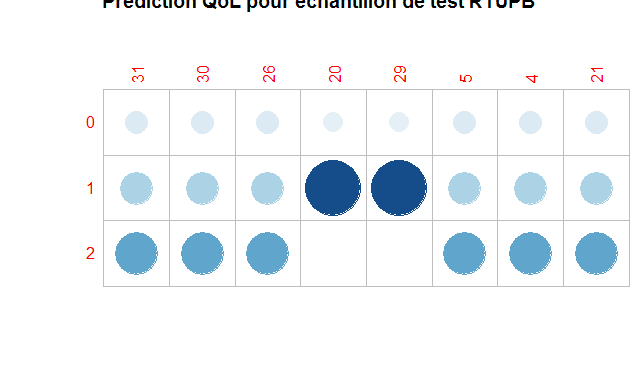
\includegraphics[width=0.75\textwidth]{../Fig/RTUPB/rtupb-regtree-predict-qol12.png}
\caption{RTUPB: Prévision pour QoL à 12 mois}
\label{fig-rtupb-regtree-predict-qol12}
\end{figure}

\begin{figure}[H]
\centering
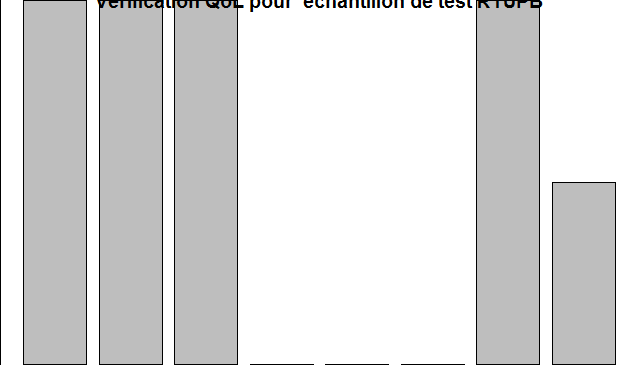
\includegraphics[width=0.75\textwidth]{../Fig/RTUPB/rtupb-regtree-test-qol12.png}
\caption{RTUPB: Valeurs Test pour QoL à 12 mois}
\label{fig-rtupb-regtree-test-qol12}
\end{figure}

En appliquant cet arbre sur l'ensemble de tests, nous obtenons pour chaque patient une table de probabilités (figure~\ref{fig-rtupb-regtree-predict-qol12}) pour chacune des valeurs QoL 0/1/2. On peut alors comparer les prédictions (les valeurs les plus probables) avec les valeurs de référence (figure~\ref{fig-rtupb-regtree-test-qol12}). Celles-ci sont correctes pour 4 patients sur 8, et incorrectes pour les 4 autres (20, 29, 5 et 21). Nous obtenons la table de correspondance suivante, entre valeurs de référence et valeurs de prédiction:

\begin{lstlisting}[language=R]
> table(validation = testQoL$QoL__4, prediction =  predict(dt, testQoL, type="class"))
           prediction
validation 0 1 2
         0 0 2 1
         1 0 0 1
         2 0 0 4
\end{lstlisting}
Soit un taux d'erreur de 50%

Afin d'améliorer les résultats de prédiction, il nous faudrait répéter l'opération et utiliser une forêt d'arbres de régression. La prédiction utilisée sera alors la prédiction moyenne de l'ensemble des arbres de la forêt. Nous obtenons alors une nouvelle table de correspondance:

\begin{lstlisting}[language=R]
> table(validation = testQoL$QoL__4, prediction =  predict(rf, testQoL))
          prediction
validation 0 1 2
         0 1 1 1
         1 0 1 0
         2 0 0 4
\end{lstlisting}
Soit un taux d'erreur moindre, de 25%

\subsubsection{RTUPB: IPSS à 12 mois}

L'arbre de régression obtenu pour la variable IPSS à 12 mois (colonne IPSS\_\_4) met en \{oe}uvre une seule variable (Cf. figure~\ref{fig-rtupb-regtree-ipss12}).
Nous vérifions le moindre rôle d'autres variables:
\begin{lstlisting}[language=R]
dt$variable.importance
            caillotage            PSA (ng/ml)              Age (ans) 
              2.992857               1.496429               1.122321 
Délai ablation (jours)               IPSS P.O                QoL P.O 
              1.122321               1.122321               1.122321 
\end{lstlisting}
Les feuilles de l'arbre représentent, en première ligne, la valeur prédite (la plus probable) pour IPSS à 12 mois. La ligne suivante indique les probabilités pour chacun des 3 niveaux constatés sur l'échantillon d'apprentissage pour IPSS à 12 mois, c'est-à-dire respectivement 1/2/3. Par exemple en cas de caillotage (valeur == 1), l'arbre de régression conduit à la feuille en bas à gauche et prédit une valeur IPSS à 1 avec une probabilité de 88\%.

En appliquant cet arbre sur l'ensemble de tests, nous obtenons pour chaque patient une table de probabilités (figure~\ref{fig-rtupb-regtree-predict-ipss12}) pour chacune des valeurs IPSS 1/2/3/4. Les prédictions (valeurs
les plus probables) sont correctes pour tous les patients à l'exception des patients 20 et 29 pour lesquels la valeur référence IPSS à 12 mois est de 1.
Nous obtenons la table de correspondance suivante, entre valeurs de référence et valeurs de prédiction:

\begin{lstlisting}[language=R]
> table(validation = testIPSS$IPSS__4, prediction =  predict(dt, testIPSS, type="class"))
           prediction
validation 1 2 3 4
         1 0 2 0 0
         2 0 6 0 0
\end{lstlisting}
Soit un taux d'erreur de 25\%

\begin{figure}[H]
\centering
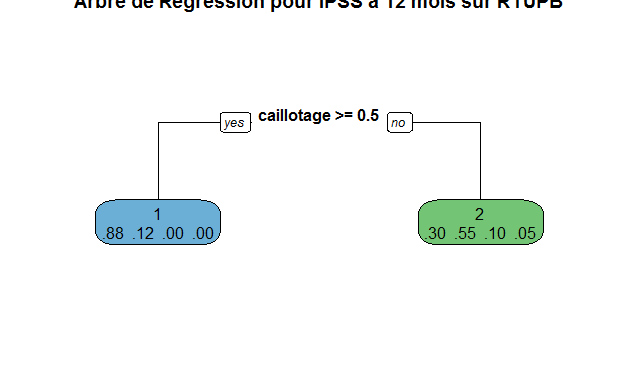
\includegraphics[width=0.75\textwidth]{../Fig/RTUPB/rtupb-regtree-ipss12.png}
\caption{RTUPB: Arbre de régression pour IPSS à 12 mois}
\label{fig-rtupb-regtree-ipss12}
\end{figure}


\begin{figure}[H]
\centering
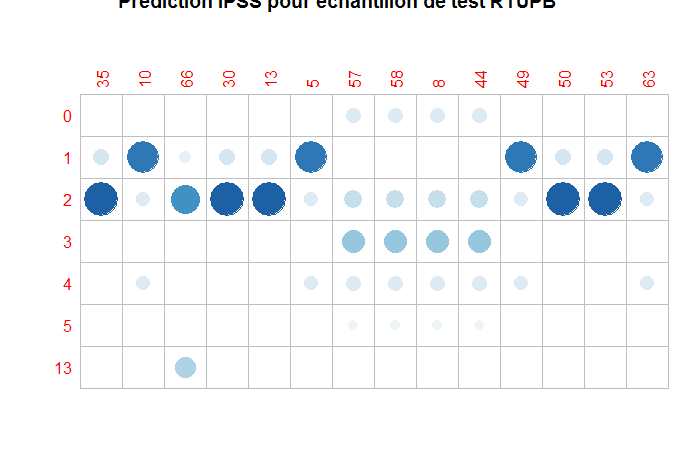
\includegraphics[width=0.75\textwidth]{../Fig/RTUPB/rtupb-regtree-predict-ipss12.png}
\caption{RTUPB: Prévision pour IPSS à 12 mois}
\label{fig-rtupb-regtree-predict-ipss12}
\end{figure}

En utilisant une forêt aléatoire d'arbres de régression, nous obtenons une nouvelle table de correspondance:
\begin{lstlisting}[language=R]
> table(validation = testIPSS$IPSS__4, prediction =  predict(rf, testIPSS))
           # prediction
# validation 1 2 3 4
         # 1 1 1 0 0
         # 2 0 4 1 1
\end{lstlisting}
Soit un taux d'erreur de 37,5\%. Si toutefois une marge d'erreur de prédiction d'un point est médicalement acceptable sur l'indice IPSS, le taux d'erreur deviendrait alors de 12,5\%.

\subsubsection{RTUPB: Qmax à 12 mois}

L'arbre de régression obtenu pour la variable Qmax à 12 mois (colonne Qmax (ml/s)\_\_3) met en oeuvre 2 variables (Cf. figure~\ref{fig-rtupb-regtree-qmax12}). Les feuilles de l'arbre représentent, en première ligne, la valeur approximative pour Qmax à 12 mois. La ligne suivante indique le nombre de patients de l'échantillon d'apprentissage correspondant à cette feuille. 

\begin{figure}[H]
\centering
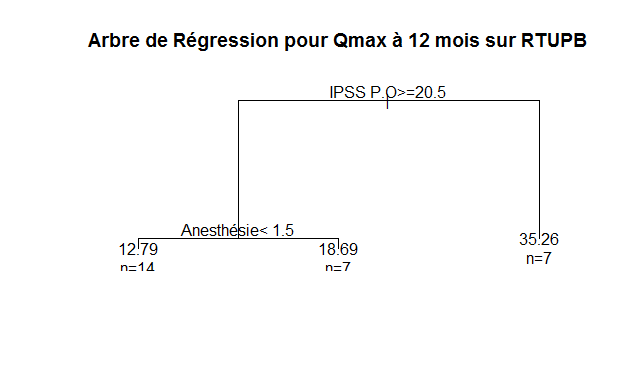
\includegraphics[width=0.75\textwidth]{../Fig/RTUPB/rtupb-regtree-qmax12.png}
\caption{RTUPB: Arbre de régression pour Qmax à 12 mois}
\label{fig-rtupb-regtree-qmax12}
\end{figure}

Pour évaluer l'arbre de régression, nous utiliserons une mesure de distance (valeur absolue de la différence) pour entre la valeur prédite et la valeur de référence pour chaque patient de l'ensemble de validation. 
La figure~\ref{fig-rtupb-regtree-test-qmax12} représente l'écart constaté entre valeurs prédites (colonne de gauche) et valeurs de référence (colonne de droite). La moyenne de ces écarts nous donne une mesure du taux d'erreur de l'arbre. En répétant l'opération pour construire une forêt d'arbres de régression, nous utiliserons alors la prédiction rendue par l'arbre avec le plus faible taux d'erreur (Cf. figure~\ref{fig-rtupb-forest-test-qmax12}).

\begin{figure}[H]
\centering
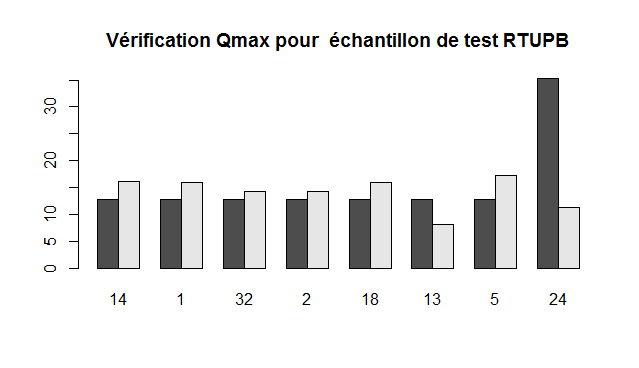
\includegraphics[width=0.75\textwidth]{../Fig/RTUPB/rtupb-regtree-test-qmax12.png}
\caption{RTUPB: Evaluation des prévisions pour Qmax à 12 mois}
\label{fig-rtupb-regtree-test-qmax12}
\end{figure}

\begin{figure}[H]
\centering
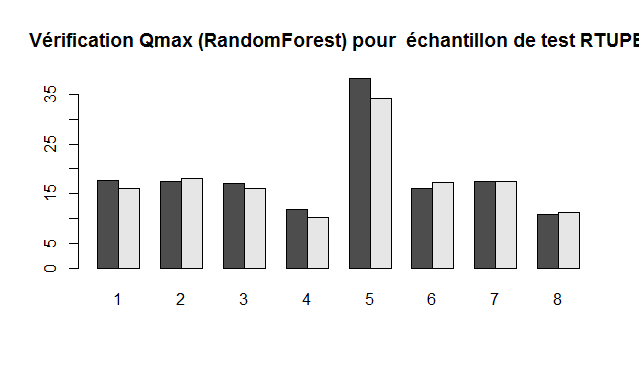
\includegraphics[width=0.75\textwidth]{../Fig/RTUPB/rtupb-forest-test-qmax12.png}
\caption{RTUPB: Evaluation des prévisions d'une forêt aléatoire pour Qmax à 12 mois}
\label{fig-rtupb-forest-test-qmax12}
\end{figure}
